
%(BEGIN_QUESTION)
% Copyright 2015, Tony R. Kuphaldt, released under the Creative Commons Attribution License (v 1.0)
% This means you may do almost anything with this work of mine, so long as you give me proper credit

Suppose a technician performs an optical power test of this optical fiber run and determines there is an excessive end-to-end power loss:

$$\includegraphics[width=15.5cm]{i02760x01.eps}$$

Assuming a typical cable attenuation of $-1$ dB per kilometer, a typical connector loss of $-2$ dB per cable-to-cable connection, and a typical fusion splice loss of $-0.2$ dB per splice, calculate the expected optical power loss for the test configuration shown.

\vskip 10pt

Describe a diagnostic procedure by which you could locate which section(s) of this optical fiber run might account for the excessive power loss.

\vskip 10pt

Identify an error the first technician may have committed that would have given a falsely high power loss measurement (i.e. explain how this fiber optic cable run might actually be within acceptable power loss parameters after all!).

\vskip 10pt

Finally, describe how an OTDR could be used to test this fiber optic run instead of an optical power meter.

\vskip 20pt \vbox{\hrule \hbox{\strut \vrule{} {\bf Suggestions for Socratic discussion} \vrule} \hrule}

\begin{itemize}
\item{} What exactly is a ``fusion splice'' and how does it differ from the ``butt connectors'' shown elsewhere in this illustration?
\item{} Identify the causes of optical power loss at connectors.
\item{} Identify the causes of optical power loss at fusion splices.
\item{} Identify the causes of optical power loss along the length of an optical fiber.
\item{} Would the result of this test be any different if we swapped locations of the optical source and power meter?  Why or why not?
\item{} What would happen to the optical power meter's reading if we were to disconnect one of the junctions in this system?
\item{} What would happen to the optical power meter's reading if we were to sharply bend one of the fibers in this system?
\end{itemize}

\underbar{file i02760}
%(END_QUESTION)





%(BEGIN_ANSWER)

 
%(END_ANSWER)





%(BEGIN_NOTES)

\noindent
Expected power loss, counting 6 connectors (although there are 7 ``butt'' connectors shown, one of these will have been ``zeroed out'' during the calibration of the optical power meter):

\vskip 10pt

($-1$ db/km)(1.2 km + 0.75 km + 2.5 km + 1 km) + ($-2$ db/connector)(6 connectors) + ($-0.2$ db/splice)(1 splice) 

\vskip 10pt

($-5.45$ db fiber loss) + ($-12$ db connector loss) + ($-0.2$ db splice loss) 

\vskip 10pt

$-17.65$ db total loss

\vskip 10pt

Therefore, the measured power loss of $-29.5$ dB is indeed excessive.

\vskip 10pt

A diagnostic procedure for pinpointing the location of the excessive power loss would involve moving the light source and/or power meter to test shorter sections of the fiber run, noting if any particular section exhibits a higher-than-normal power loss.

\vskip 10pt

It is possible the technician committed an error in the initial power measurement, by not properly ``zeroing'' the optical power meter before testing the cable.

\vskip 10pt

An OTDR could test this cable all from one end, giving a complete characterization of all losses and their locations along the fiber run!



%INDEX% Electronics review: fiber optics

%(END_NOTES)


